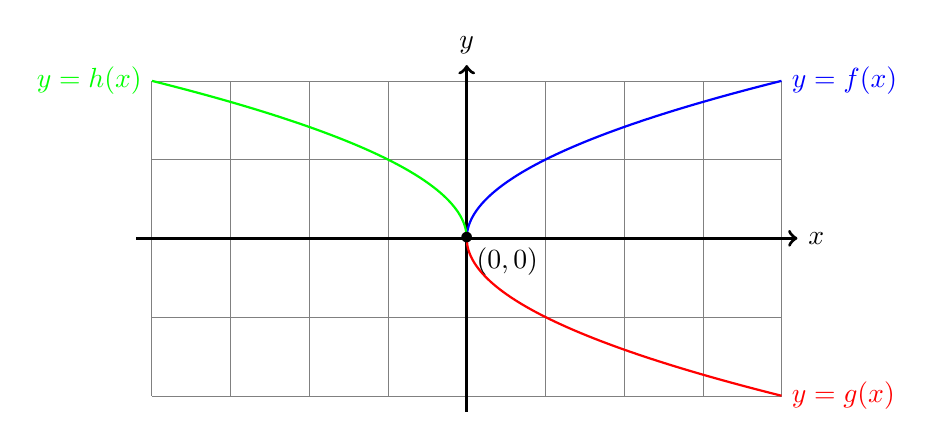
\begin{tikzpicture}
  \draw[very thin,color=gray] (-4,-2) grid (4,2);

  \draw[very thick,->] (-4.2,0) -- (4.2,0) node[right] {$x$};
  \draw[very thick,->] (0,-2.2) -- (0,2.2) node[above] {$y$};
  
  \draw [color=blue,thick] plot[smooth,samples=500,domain=0:4] (\x,{sqrt(\x)}) node [right] {$y = f(x)$};
  \draw [color=red,thick] plot[smooth,samples=500,domain=0:4] (\x,{-sqrt(\x)}) node [right] {$y = g(x)$};
  \draw [color=green,thick] plot[smooth,samples=500,domain=0:-4] (\x,{sqrt(-\x)}) node [left] {$y = h(x)$};

  \node at (0,0) {$\bullet$};
  \node [below right] at (0,0) {$(0,0)$};
\end{tikzpicture}
